Modelling human-generated ``random" data is notoriously difficult. In this project, we attempted to model the behavior of one user of twitter using various random processes. The user was observed over the course of around 6 months posting (emitting) a little over 3,300 tweets. The goal is to find some kind of model to fit these data, without using a hideously large number of parameters.

The data are visualised in Figure \ref{raw_data}. We see a little seasonality - the user seems to be going to sleep at some time, waking up at another time - but beyond that we'll be reliant on statistical tests to judge how good our model is.

\begin{figure}[h]
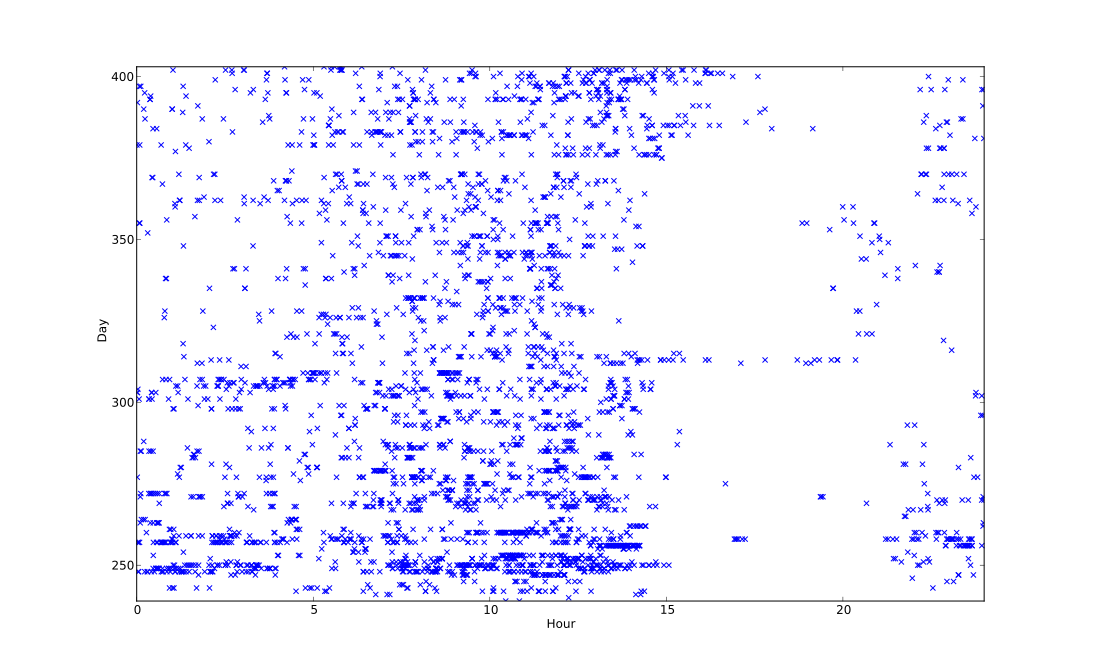
\includegraphics[width = \textwidth]{./images/raw_data.png}
\caption{The raw data gathered from the twitter user. Each blue cross marks a tweet at a particular time.}
\label{raw_data}
\end{figure}